\documentclass[11pt]{article}
\usepackage{geometry} % Pour passer au format A4
\geometry{hmargin=1cm, vmargin=1cm} % 

% Page et encodage
\usepackage[T1]{fontenc} % Use 8-bit encoding that has 256 glyphs
\usepackage[english,french]{babel} % Français et anglais
\usepackage[utf8]{inputenc} 

\usepackage{lmodern}
\setlength\parindent{0pt}

% Graphiques
\usepackage{graphicx,float,grffile}
\usepackage{pst-eucl, pst-plot,units} 

% Maths et divers
\usepackage{amsmath,amsfonts,amssymb,amsthm,verbatim}
\usepackage{multicol,enumitem,url,eurosym,gensymb}

% Sections
\usepackage{sectsty} % Allows customizing section commands
\allsectionsfont{\centering \normalfont\scshape}

% Tête et pied de page

\usepackage{fancyhdr} 
\pagestyle{fancyplain} 

\fancyhead{} % No page header
\fancyfoot{}

\renewcommand{\headrulewidth}{0pt} % Remove header underlines
\renewcommand{\footrulewidth}{0pt} % Remove footer underlines

\newcommand{\horrule}[1]{\rule{\linewidth}{#1}} % Create horizontal rule command with 1 argument of height

%----------------------------------------------------------------------------------------
%   Début du document
%----------------------------------------------------------------------------------------

\begin{document}

%----------------------------------------------------------------------------------------
% RE-DEFINITION
%----------------------------------------------------------------------------------------
% MATHS
%-----------

\newtheorem{Definition}{Définition}
\newtheorem{Theorem}{Théorème}
\newtheorem{Proposition}{Propriété}

% MATHS
%-----------
\renewcommand{\labelitemi}{$\bullet$}
\renewcommand{\labelitemii}{$\circ$}
%----------------------------------------------------------------------------------------
%   Titre
%----------------------------------------------------------------------------------------

\setlength{\columnseprule}{1pt}

\horrule{2px}
\section*{Chapitre - Thalès}
\horrule{2px}

\section*{I - Démonstration}

\subsection*{1 - Proportionnalité}

\begin{multicols}{2}

  Pour trouver les valeurs manquantes dans un tableau de proportionnalité, on fait \textbf{le produit en croix}.

  \begin{center}
    \begin{tabular}{|c|c|c|}
      \hline
      12 &  & 26 \\  \hline
      24 & 96 &  \\  \hline
    \end{tabular}
  \end{center}

  On calcule les produit en croix suivant :

  \begin{itemize}
    \item $12 \times 96 \div 24 = 48$
    \item $24 \times 26 \div 12 = 52$
  \end{itemize}

\end{multicols}

Le sens du tableau de proportionnalité est une égalité de rapport :

\begin{multicols}{2}

  \begin{center}
    \begin{tabular}{|c|c|c|}
      \hline
      12 & 48 & 26 \\  \hline
      24 & 96 & 52 \\  \hline
    \end{tabular}
  \end{center}

  \begin{center} $\dfrac{12}{24} = \dfrac{48}{96} = \dfrac{26}{52}$ \end{center}

\end{multicols}

D'ailleurs pour vérifier qu'un tableau est proportionnel, on vérifie chacun de ses rapports :

$\dfrac{12}{24} = 0.5$ ; $\dfrac{48}{96} = 0.5 \text{ et } \dfrac{26}{52} = 0.5$

\subsection*{2 - Triangles semblables}

\begin{Definition}
  Deux triangles semblables ont des angles de même mesures. \og Ils ont la même forme.\fg
\end{Definition}

\begin{Proposition}
  Des triangles semblables ont des côtés deux à deux proportionnels.
\end{Proposition}

\begin{figure}[H]
  \centering
  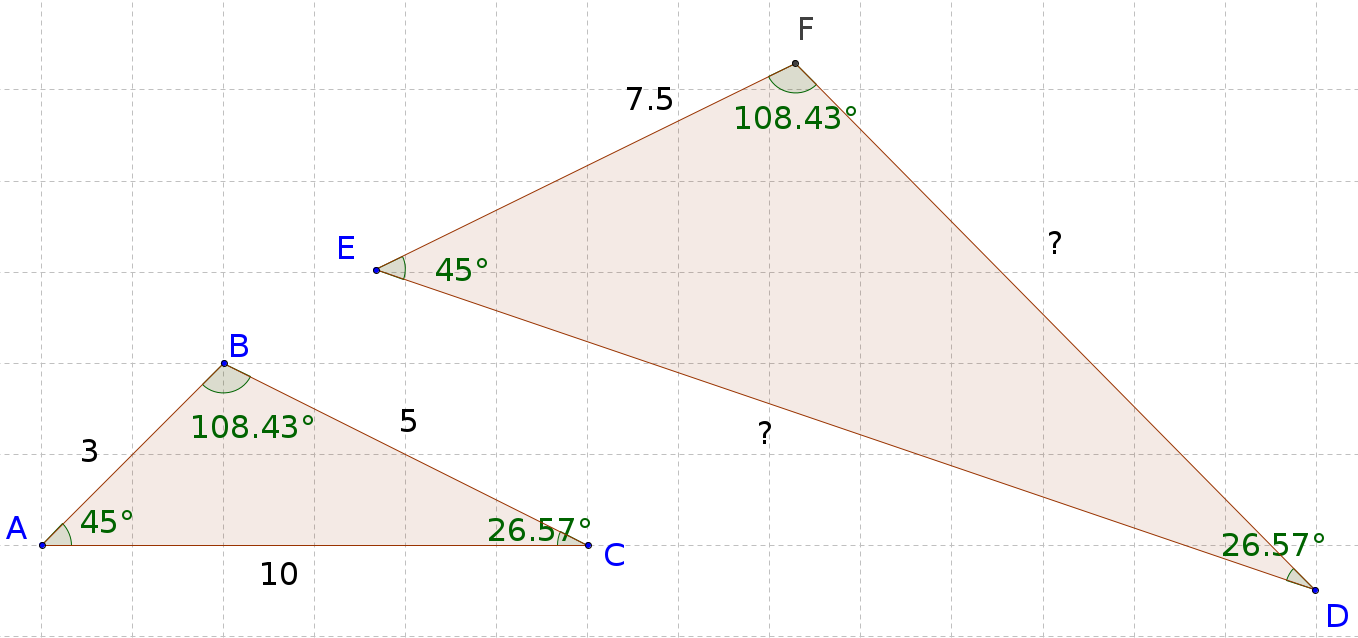
\includegraphics[width=0.6\linewidth]{3x6-thales/sources/tri-sem.png}
\end{figure}

Si on a deux triangles semblables, on peut calculer les longueurs de l'un à partir des longueurs de l'autre. On utilise le tableau de proportionnalité et le produit en croix.

\begin{multicols}{2}

  \begin{center}
    \begin{tabular}{|l|c|c|c|}
      \hline
      Premier triangle  : ABC & AB & BC  & AC \\  \hline
      Deuxième triangle : EFD & EF & FD & ED \\  \hline
    \end{tabular}
  \end{center}

  \begin{center}
    \begin{tabular}{|l|c|c|c|}
      \hline
      Premier triangle  : ABC & 3   & 5  & 10 \\  \hline
      Deuxième triangle : EFD & 7.5 & FD & ED \\  \hline
    \end{tabular}
  \end{center}

  On trouve à l'aide du produit en croix :

  \begin{itemize}
    \item $FD = 5 \times 7.5 \div 3 = 12.5$
    \item $ED = 10 \times 7.5 \div 3 = 25$
  \end{itemize}

\end{multicols}

\newpage
\subsection*{3 - Angles et parallélisme}

\subsubsection*{Angles correspondants}

  \begin{figure}[H]
    \centering
    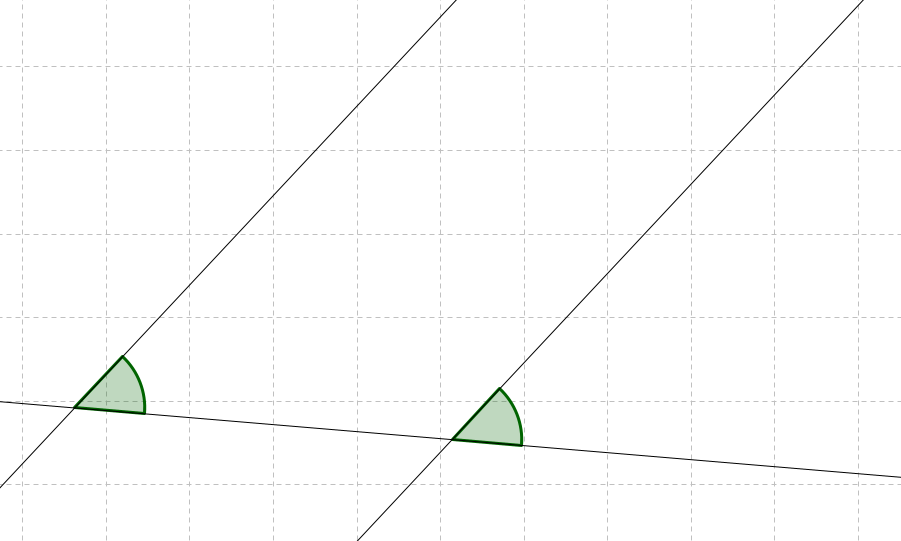
\includegraphics[width=0.3\linewidth]{3x6-thales/sources/dr-1.png}
  \end{figure}

  \begin{center}Des angles correspondants sont égaux si les droites sont parallèles. \end{center}

  \begin{figure}[H]
    \centering
    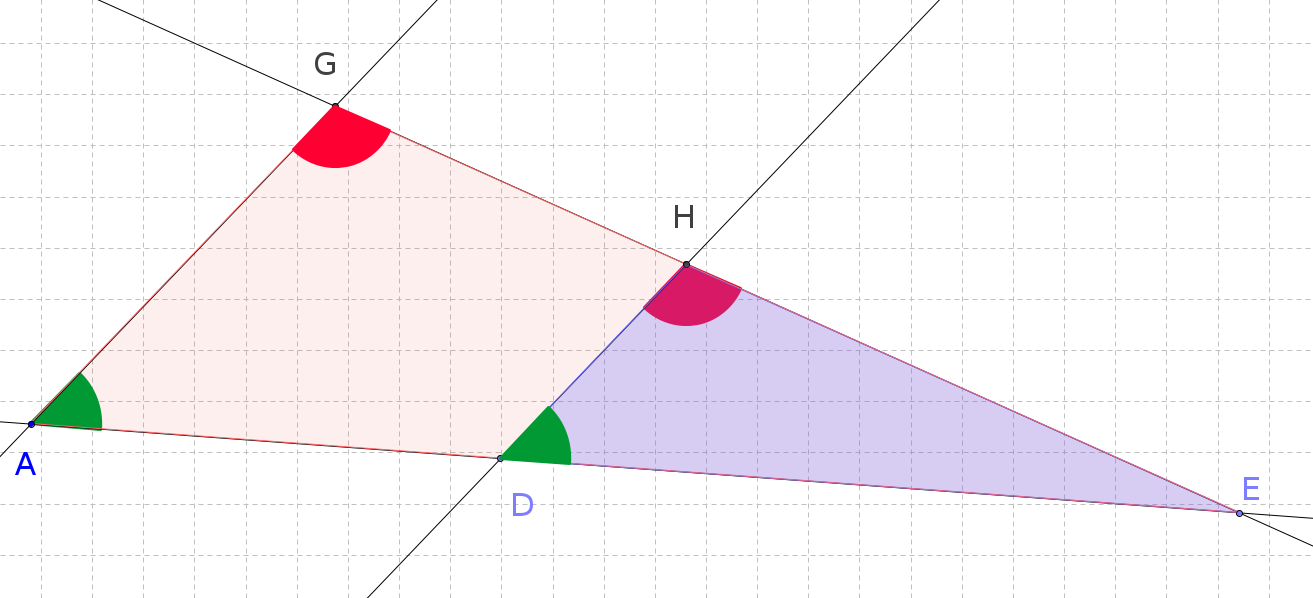
\includegraphics[width=0.5\linewidth]{3x6-thales/sources/dr-2.png}
  \end{figure}

  \begin{center}Si les droites sont parallèles alors les triangles sont semblables.\end{center}



\subsubsection*{Angles opposés et Alternes-internes}

\begin{center}
\begin{multicols}{2}

  \begin{figure}[H]
    \centering
    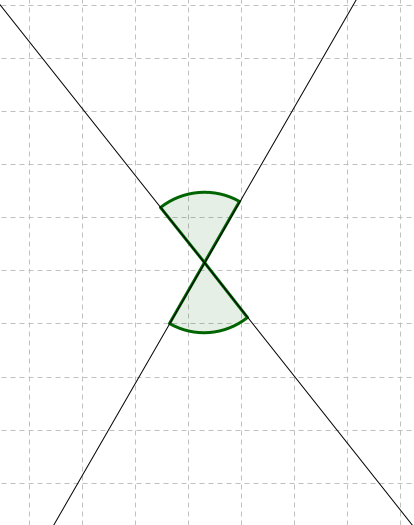
\includegraphics[width=0.3\linewidth]{3x6-thales/sources/dr-3.png}
  \end{figure}

  Des angles opposés par le sommet sont égaux.\columnbreak

  \begin{figure}[H]
    \centering
    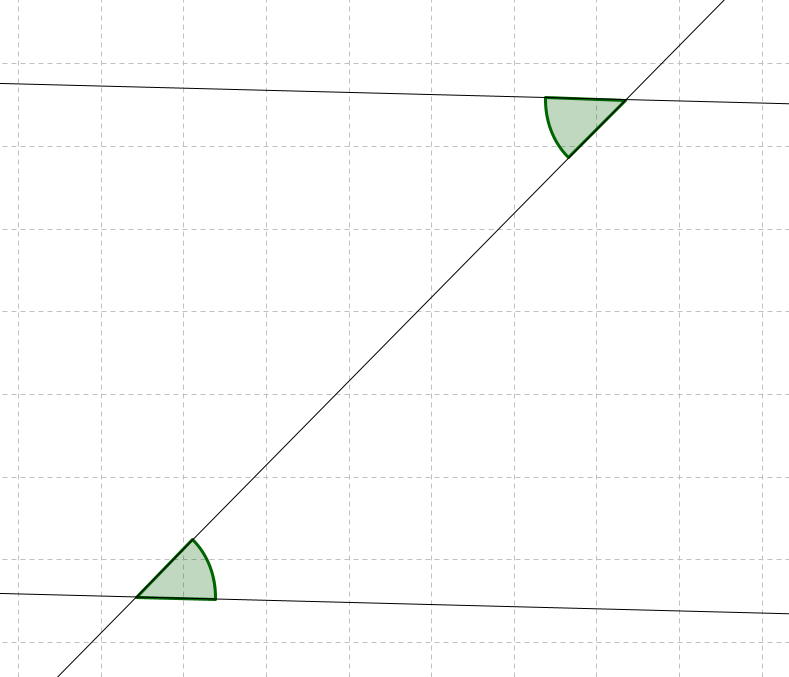
\includegraphics[width=0.5\linewidth]{3x6-thales/sources/dr-4.png}
  \end{figure}

Des angles alternes-internes sont égaux si les droites sont parallèles. 

\end{multicols}

\begin{figure}[H]
  \centering
  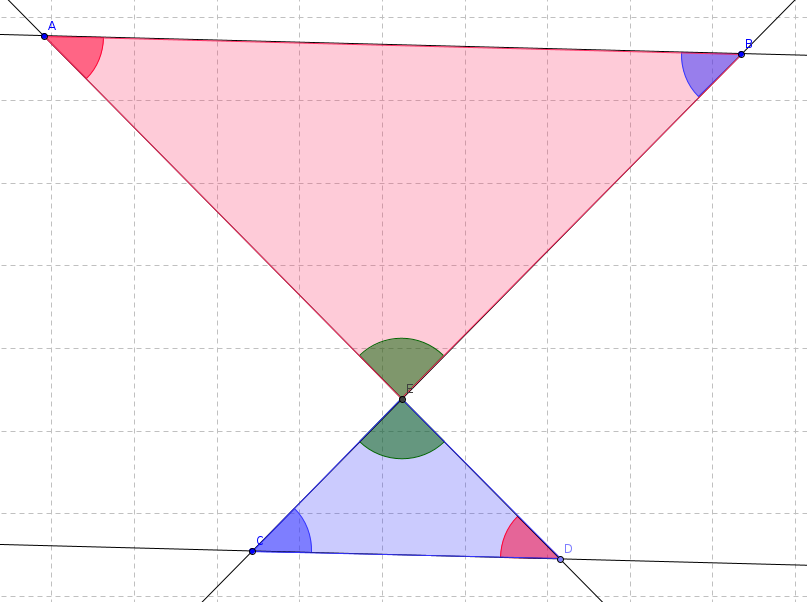
\includegraphics[width=0.3\linewidth]{3x6-thales/sources/dr-5.png}
\end{figure}

Si les droites sont parallèles alors les triangles sont semblables.
\end{center}

\newpage
\subsection*{4 - Théorème de Thalès vs Triangles Semblables}

Il est parfois compliqué de démontrer que deux triangles sont semblables. On n'a rarement toutes les données d'angles.  \\

Par contre dans le cas où des droites sont parallèles, on arrive facilement à ce résultat. \textbf{Le théorème de Thalès} est un cas particulier de la propriété des triangles semblables si on a une configuration avec \textbf{des droites parallèles.} Les conditions d'utilisation du théorème sont plus simples. 

\section*{II - Usages}

Le théorème de Thalès est utilisé dans deux types d'exercice.

\begin{itemize}
  \item Le sens direct est le calcul de longueurs manquantes si a des droites parallèles.  
  \item La réciproque est la démonstration du parallélisme si on connaît suffisamment de longueurs.
\end{itemize}



\subsection*{1 - Calcul de longueurs}

\begin{multicols}{2}

  \subsubsection*{ÉNONCÉ}

  Sur la figure ci-dessous, les droites $(YO)\text{ et }(UG)$ sont parallèles.

  On donne $RO=\unit[5,4]{cm}$, $YO=\unit[5,2]{cm}$, $RU=\unit[2,3]{cm}$ et $UG~= \unit[2,7]{cm}$. \\
  \textbf{Calculer $RY$ et $RG$.}

  \begin{figure}[H]
          \centering
          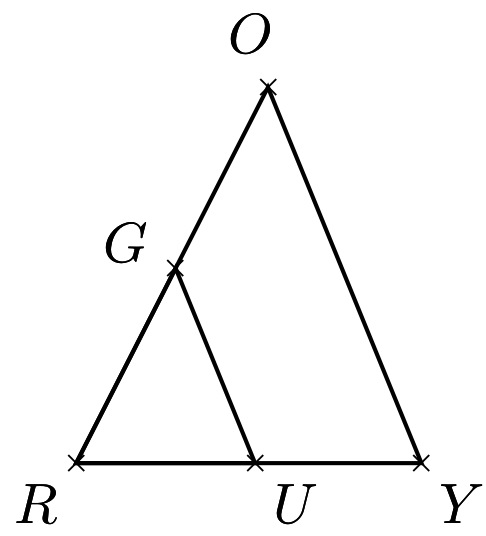
\includegraphics[width=0.4\linewidth]{3x6-thales/sources/thales-1.png}
    \end{figure}
  \columnbreak

  \subsubsection*{RÉDACTION}
  
  \begin{itemize}
    \item Les points $R$,~ $U$,~ $Y$ et $R$, $G$, $O$ sont alignés.
    \item Les droites $(YO)$ et $(UG)$ sont parallèles.
    \item D'après le \textbf{théorème de Thalès} : $\mathbf{\cfrac{RY}{RU}=\cfrac{RO}{RG}=\cfrac{YO}{UG}}$
    \item $\dfrac{RY}{2,3}=\dfrac{5,4}{RG}=\dfrac{5,2}{2,7}$\\
  \end{itemize}

  \textbf{CALCULS :} \\

  $\cfrac{5{,}2}{2{,}7}=\cfrac{RY}{2{,}3} \quad$ donc $\quad \boxed{RY=\cfrac{2{,}3\times 5{,}2}{2{,}7}\simeq\unit[4{,}429]{cm}}$ \newline
  $\cfrac{5{,}2}{2{,}7}=\cfrac{5{,}4}{RG} \quad$ donc $\quad \boxed{RG=\cfrac{5{,}4\times 2{,}7}{5{,}2}\simeq\unit[2{,}803]{cm}}$
   
\end{multicols}

\subsection*{2 - parallélisme}

\begin{multicols}{2}

  \subsubsection*{ÉNONCÉ}

  \begin{figure}[H]
    \centering
    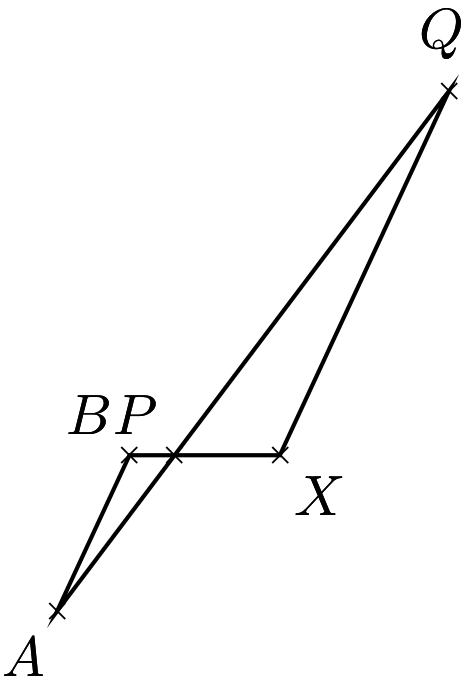
\includegraphics[width=0.4\linewidth]{3x6-thales/sources/thales-2.png}
  \end{figure}

  Sur la figure ci-contre, on donne $PQ=\unit[18,2]{cm}$, $PX=\unit[4,2]{cm}$, $AQ=\unit[26]{cm}$ et $PB=\unit[1,8]{cm}$.\\
  \textbf{Démontrer que les droites $(XQ)$ et $(BA)$ sont parallèles.}
  \columnbreak
    
  \subsubsection*{RÉDACTION}
    Les points $B$, $P$, $X$~ et $A$, $P$, $Q$ sont alignés dans le même ordre. \\
    De plus $PA=AQ-PQ=\unit[7,8]{cm}$.

    \begin{itemize}
      \item $\cfrac{PX}{PB}=\cfrac{4,2}{1,8}=\cfrac{7}{3}$
      \item $\cfrac{PQ}{PA}=\cfrac{18,2}{7,8}=\cfrac{7}{3}$ \\
    \end{itemize}

    Donc $\cfrac{PX}{PB}=\cfrac{PQ}{PA}$.\\

    D'après la \textbf{réciproque du théorème de Thalès}, \fbox{les droites $(XQ)$ et $(BA)$ sont parallèles.}
\end{multicols}

\end{document}
